\begin{enumerate}
\item Cual la diferencia entre un SGBD  Mono Usuario y un SGBD Multiusuario?

Un sistema gestor de base de datos monousario, son sistemas gestores que solo son utilizados por un usuario a la vez. Por otro lado, los multiusarios son sistemas gestores que pueden ser utilizados por varios usuarios a la vez.

\item Explique el concepto de Multiprogramación en los Sistema Operativos.

También llamado sistemas operativos multitarea o multiproceso, se distingue por la habilidad de soportar dos o más procesos activos simultáneamente. Eltérmino multiprogramación denota un sistema operativo que, además de soportar procesos concurrentes múltiples, permite que residan simultáneamente en la memoria primaria las instrucciones y los datos procedentes de dos o más procesos distintos.

\item Explique los conceptos de Concurrencia Intercalada y Paralela.

La concurrencia intercalada, consiste en ejecutar las transacciones de forma intercalada, esta forma de ejecutar suele traer inconsistencia a la base de datos.Mientras que concurrencia Paralela, consiste en ejecutar las transacciones una después de la otra, esta forma de ejecutar trae a la base de datosuna consistencia segura

\item Explique el concepto de Transacciones Concurrentes

Se le llama así cuando varias transacciones introducidas por usuarios, seejecutan de manera simultánea, pudiendo leer/modificar el mismo elemento de la base de datos

\item Dadas dos transacciones T1 y T2, explique las dos formas posible que tiene el SGBD para ejecutar ambas transacciones.

\begin{table}[ht!]
\begin{center}
\begin{tabular}{|l|l|}
\hline
\multicolumn{1}{|c|}{T1}                                                                                        & \multicolumn{1}{c|}{T2}                                                    \\ \hline
\begin{tabular}[c]{@{}l@{}}leer (X);\\ X:= X-N;\\ escribir(X);\\ leer(Y);\\ Y:=Y+N;\\ escribir(Y);\end{tabular} & \begin{tabular}[c]{@{}l@{}}leer(X);\\ X:= X+M;\\ escribir(X);\end{tabular} \\ \hline
\end{tabular}
\end{center}
\end{table}
Una manera de realizar las dos transacciones es realizarlas de manera paralela, ejecutando primero T1, seguido por T2. La segunda manera es realizar T1 y T2 de forma intercalada.

\item Cite algunas razones por la cual es importante la ejecución concurrente de dos o más transacciones.

\begin{itemize}
\item Aumenta la productividad: número de transacciones ejecutadas por minuto
\item Aumenta la utilización de la CPU(menos tiempo de ociosa) y control de Disco
\item Reducir el tiempo medio de respuesta de transacciones
\end{itemize}

\item  Las transacciones concurrentes deben controlar dos operaciones. ¿Cuáles son?

Deben controlar la lectura de datos y las modificaciones de datos de la base de datos.

\item  Defina el concepto de lectura de valor Fantasma en las Transacciones

Esto ocurre cuando, durante una transacción, se ejecutan dos consultas idénticas, y los resultados de la segunda son distintos de los de la primera.Esto puede ocurrir cuando no se realizan los bloqueos de rango al realizar la operación \texttt{SELECT... WHERE}

\item  Defina el concepto de lectura de valor Sucio en las Transacciones

Una lectura sucia ocurre cuando se le permite a una transacción la lectura de una fila que ha sido modificada por otra transacción concurrente pero todavía no ha sido cometida.Las lecturas sucias funcionan de modo similar a las lecturas no repetibles, sin embargo la segunda transacción no necesita ser cometida para que la primera de un resultado diferente.

\item  Cite por lo menos 3 ejemplos que ocasiona ejecutar Transacciones Concurrentes.

\begin{itemize}
\item Guardar una cantidad de asientos para un concierto.
\item Hacer depósito a otras cuentas de diferentes lugares y de manera simultánea.
\item Sistema de Base de Datos que permita hacer y anular reservas de asientos en vuelos de diferentes compañías aéreas.
\end{itemize}

\item En los SGBD ¿Cual es función del Planificador de Transacciones?.

Es la de controlar el acceso concurrente y específicamente de transacciones concurrentes.El planificador crea agenda, secuencias ordenadas de las operaciones de Lectura/Escritura tomadas por una o más transacciones.

\item Que es el Protocolo de Control de Concurrencia?

Los protocolos de control de concurrencia son reglas acerca de cómo se deben acceder los recursos para generar planificaciones secuenciales.

\item Cuál es el objetivo del Protocolo de Control de Concurrencia

\begin{itemize}
\item Planificar las transacciones de forma que no ocurran interferencias entre ellas, y así evitar la aparición de problemas.
\item Solución obvia: no permitir intercalación de operaciones de varias transacciones.
\end{itemize}

\item  Si los SGBD permiten ejecutar de manera intercalas las instrucciones de T1 y T2, cite por lo menos tres formas de ejecutar ambas transacciones.

\begin{table}[ht!]
\begin{center}
\begin{tabular}{|l|l|}
\hline
\multicolumn{1}{|c|}{T1}                                                                                        & \multicolumn{1}{c|}{T2}                                                    \\ \hline
\begin{tabular}[c]{@{}l@{}}leer (X);\\ X:= X-N;\\ escribir(X);\\ leer(Y);\\ Y:=Y+N;\\ escribir(Y);\end{tabular} & \begin{tabular}[c]{@{}l@{}}leer(X);\\ X:= X+M;\\ escribir(X);\end{tabular} \\ \hline
\end{tabular}
\end{center}
\end{table}
\begin{itemize}
\item $P_A:$\texttt{ l2(X);e1(X);  l1(Y); e2(X); c2; e1(Y); c1 ;} 
\item $P_B:$\texttt{l1(X) ; e1(X) ; l1(Y) ; e1(Y) ; c1 ; l2(X) ; e2(X) ; c2 ;}
\item $P_C:$\texttt{ l1(X) ; l2(X) ; e2(X) ; c2 ; l1(X) ; e1(X) ; l1(Y) ; e1(Y) ; c1 ;}
\end{itemize}
\item Que es una Planificación de Transacciones y que condiciones debe cumplirse.

Es una secuencia de las operaciones realizadas por dichas transacciones, sujeta a la restricción de que:
\begin{itemize}
\item Para cada transacción Ti, que participa en P,
\item Sus operaciones aparecen en P
\item En el mismo orden en el que ocurren en Ti.
\end{itemize}

\item La tabla 1 especifica la abreviación de las operaciones que participan en una Transacción,  usando la tabla 1 se escriben las planificaciones $P_A$ y $P_B$, escriba otras posibles planificaciones $P_C$, $P_D$ y $P_E$. (El subíndice de cada operación indica a la transacción que pertenece)

\begin{itemize}
\item $P_A$: \texttt{l1(X) ; e1(X) ; l1(Y) ; e1(Y) ; c1 ; l2(X) ; e2(X) ; c2 ;}

\item $P_B$: \texttt{l2(X) ; e2(X) ; c2 ; l1(X) ; e1(X) ; l1(Y) ; e1(Y) ; c1 ;}

\item $P_C$: \texttt{l1(X) ; l2(X) ; e1(X) ; l1(Y) ; e2(X) ; c2 ; e1(Y) ; c1;}

\item $P_D$: \texttt{l1(X) ; e1(X) ; l2(X) ; e2(X) ; c2; l1(Y) ; e1(Y) ; c1 ;}

\begin{table}[ht!]
\begin{center}
\begin{tabular}{|l|l|}
\hline
\multicolumn{1}{|c|}{operacion}                                             & \multicolumn{1}{c|}{abreviatura}                      \\ \hline
\begin{tabular}[c]{@{}l@{}}leer\\ escribir\\ commit\\ rollback\end{tabular} & \begin{tabular}[c]{@{}l@{}}l\\ e\\ c\\ r\end{tabular} \\ \hline
\end{tabular}
\end{center}
\end{table}

\begin{table}[ht!]
\begin{center}
\begin{tabular}{|l|l|}
\hline
\multicolumn{1}{|c|}{T1}                                                                                        & \multicolumn{1}{c|}{T2}                                                    \\ \hline
\begin{tabular}[c]{@{}l@{}}leer (X);\\ X:= X-N;\\ escribir(X);\\ leer(Y);\\ Y:=Y+N;\\ escribir(Y);\end{tabular} & \begin{tabular}[c]{@{}l@{}}leer(X);\\ X:= X+M;\\ escribir(X);\end{tabular} \\ \hline
\end{tabular}
\end{center}
\end{table}
\end{itemize}

\item Para las transacciones T1 y T2 ¿Cuál de las siguientes planificaciones son correctas y cuáles no?. Indicar en cada caso por qué.
\begin{itemize}

\item $P_A$: \texttt{l1(X) ; e1(X); l1(Y); e1(Y); c1 ; l2(X) ; e2(X) ; c2 ;} \\ \textbf{Correcta}, porque esta se realiza de manera secuencial y así no deja a la base de datos inconsistente

\item $P_B$: \texttt{e1(Y); l1(X) ; l1(Y); e1(X) ; c1 ; e2(X) ; l2(X) ; c2 ;} \\ \textbf{Incorrecta}, porque el orden en el que se ejecutan las transacciones no es el mismo orden en el que está escrito

\item $P_C$: \texttt{l2(X); c2; l1(X); e1(X);e1(Y); c1 ;} \\ \textbf{Incorrecta}, porque no están todas las ejecuciones de las transacciones

\item $P_D$: \texttt{l2(X); e2(X); c2; l1(X);e1(X);l1(Y); e1(Y) ; c1 ;} \\ \textbf{Correcta}, porque se ejecuta de manera secuencial
\end{itemize}

\begin{table}[ht!]
\begin{center}
\begin{tabular}{|l|l|}
\hline
\multicolumn{1}{|c|}{T1}                                                                                        & \multicolumn{1}{c|}{T2}                                                    \\ \hline
\begin{tabular}[c]{@{}l@{}}leer (X);\\ X:= X-N;\\ escribir(X);\\ leer(Y);\\ Y:=Y+N;\\ escribir(Y);\end{tabular} & \begin{tabular}[c]{@{}l@{}}leer(X);\\ X:= X+M;\\ escribir(X);\end{tabular} \\ \hline
\end{tabular}
\end{center}
\end{table}

\item Defina el concepto de Planificación Serie

Es aquella en la que las operaciones de cada transacción se ejecutan consecutivamente sin que se intercalen las operaciones de otras transacciones.

\item Defina el concepto de Planificación No Serie

Es aquella en la que las operaciones de un conjunto de transacciones concurrentes se ejecutan intercaladas.

\item Cual la diferencia entre Planificación Serie y Planificación No serie

La diferencia es que la planificación serie se ejecuta de manera consecutiva y la planificación no serie se ejecuta de manera intercalada.

\item Para las transacciones T1 y T2 ¿Cuál de las siguientes planificaciones son Serie y cuáles no?. Indicar en cada caso por qué.

\begin{itemize}
\item $P_A$  : \texttt{l1(X) ; e1(X) ; l2(X) ; e2(X) ; c2 ; l1(Y) ; e1(Y) ; c1 ;} \\Es planificación no serie, ya que se ejecuta de manera intercalada

\item $P_B$: \texttt{l1(X) ; e1(X) ; l2(X) ; e2(X) ; l1(Y) ; c2 ; e1(Y) ; c1 ;} \\ Es planificación no serie, ya que se ejecuta de manera intercalada.

\item $P_C$: \texttt{l1(X) ; e1(X) ; l2(X) ; e2(X) ; l1(Y) ; e1(Y) ; c2 ; c1 ;} \\ Es planificación no serie, ya que se ejecuta de manera intercalada.

\item $P_D$: \texttt{l1(X) ; e1(X) ; l2(X) ; e2(X) ; l1(Y) ; e1(Y) ; c1 ; c2 ;} \\ Es planificación no serie, ya que se ejecuta de manera intercalada.

\item $P_E$:\texttt{ l1(X) ; e1(X) ; l2(X) ; l1(Y) ; e2(X) ; e1(Y) ; c1 ; c2 ;} \\ Es planificación no serie, ya que seejecuta de manera intercalada.

\item $P_F$: \texttt{l1(X) ; e1(X) ; l2(X) ; l1(Y) ; e1(Y) ; e2(X) ; c1 ; c2 ;} \\ Es planificación no serie, ya que se ejecuta de manera intercalada.

\item $P_G$: \texttt{l1(X) ; e1(X) ; l2(X) ; l1(Y) ; e1(Y) ; c1 ; e2(X) ; c2 ;} \\ Es planificación no serie, ya que se ejecuta de manera intercalada.

\item $P_H$: \texttt{l1(X) ; e1(X) ; l1(Y) ; l2(X) ; e1(Y) ; c1; e2(X) ; c2 ;} \\ Es planificación no serie, ya que seejecuta de manera intercalada.

\item $P_I$: \texttt{l1(X) ; e1(X) ; l1(Y) ; e1(Y) ; l2(X) ; c1 ; e2(X) ; c2 ;} \\ Es planificación no serie, ya que se ejecuta de manera intercalada.

\item $P_J$: \texttt{l1(X) ; e1(X) ; l1(Y) ; e1(Y) ; c1 ; l2(X) ; e2(X) ; c2 ;} \\ Es planificación serie, ya que se ejecuta de manera consecutiva.
\end{itemize}

\begin{table}[ht!]
\begin{center}
\begin{tabular}{|l|l|}
\hline
\multicolumn{1}{|c|}{T1}                                                                                        & \multicolumn{1}{c|}{T2}                                                    \\ \hline
\begin{tabular}[c]{@{}l@{}}leer (X);\\ X:= X-N;\\ escribir(X);\\ leer(Y);\\ Y:=Y+N;\\ escribir(Y);\end{tabular} & \begin{tabular}[c]{@{}l@{}}leer(X);\\ X:= X+M;\\ escribir(X);\end{tabular} \\ \hline
\end{tabular}
\end{center}
\end{table}

\item Que es un Plan Equivalente

Es aquel que produce los mismos efectos en la Base de Datos

\item Defina el concepto de Planificación Serializable.

Una planificación es serializable si es equivalente a alguna planificación serie de la misma n transacciones.

\item Existen dos manera de definir la Equivalencia entre Transacciones ¿Cuáles son?

Por conflictos y por series.

\item Explique ¿Cuándo dos operaciones de una Planificación están en conflicto?. Cite ejemplos.

Están en conflicto si pertenecen a diferentes transacciones, tienen acceso al mismo elemento leer(x), y al menos una de ellas es escribir(x).

\begin{itemize}
\item P: \texttt{l1(X) ; e2(X) ;}
\item P: \texttt{e1(X) ; e2(X) ;}
\item P: \texttt{e1(X) ; l2(X) ;}
\end{itemize}


\item Dada la siguientes Planificaciones, indicar cuales operaciones están en conflicto, para cada caso explicar por qué.

$P_A$: \texttt{l1(X) ; l2(X) ; e1(X) ; l1(Y) ; e2(X) ; c2; e1(Y) ; c1;}
\\
Está en conflicto porque está leyendo un mismo elemento y también escribiendo el mismo elemento antes de que haya un commit en alguna de las dos transacciones.

$P_B$: \texttt{l1(X) ; e1(X) ; l2(X) ; e2(X) ; c2; l1(Y) ; e1(Y) ; c1;} Están en conflicto la transacción T2 puede que este leyendo un dato sucio.

\item ¿Cuándo un Plan No Serie es equivalentes por conflictos?

Son equivalentes si el orden de cualesquiera, dos operaciones en conflicto es el mismo en ambos planes.

\item Dada la siguientes Planificación No Serie  PD, validar paso a paso si la misma es equivalente por Conflicto.

PD: l1(X) ; e1(X) ; l2(X) ; e2(X) ; c2; l1(Y) ; e1(Y) ; c1;

PD1: l1(X) ; e1(X) ; l2(X) ; e2(X) ; l1(Y) ; c2; e1(Y) ; c1;

PD2: l1(X) ; e1(X) ; l2(X) ; e2(X) ; l1(Y) ; e1(Y) ; c2 ; c1;

PD3: l1(X) ; e1(X) ; l2(X) ; e2(X) ; l1(Y) ; e1(Y) ; c1; c2 ; 

PD4: l1(X) ; e1(X) ; l2(X) ; l1(Y) ; e2(X); e1(Y) ; c1; c2 ; 

PD5: l1(X) ; e1(X) ; l2(X) ; l1(Y) ; e1(Y) ; e2(X); c1 ; c2 ; 

PD6: l1(X) ; e1(X) ; l2(X) ;l1(Y) ; e1(Y) ; c1; e2(X) ; c2 ; 

PD7: l1(X) ; e1(X) ; l1(Y) ; l2(X) ;e1(Y) ; c1; e2(X) ; c2 ; 

PD8: l1(X) ; e1(X) ; l1(Y) ; e1(Y) ; l2(X) ;c1 ; e2(X) ; c2 ; 

PD9: l1(X) ; e1(X) ; l1(Y) ; e1(Y) ; c1; l2(X) ; e2(X) ; c2 ;

\item Describa los pasos del Algoritmo (usando grafos) que permite determinar si un Plan es serializable por conflictos.

Una arista Ti ->Tk indica que Tidebe aparecer antes de Tk en una planificación serie equivalente a P, pues dos operaciones en conflicto aparecen en dicho orden P.Si el grafo contiene un ciclo, P no es serializable, por conflictos.Si no hay cliclos en el grafo, P es serializable.

\begin{center}
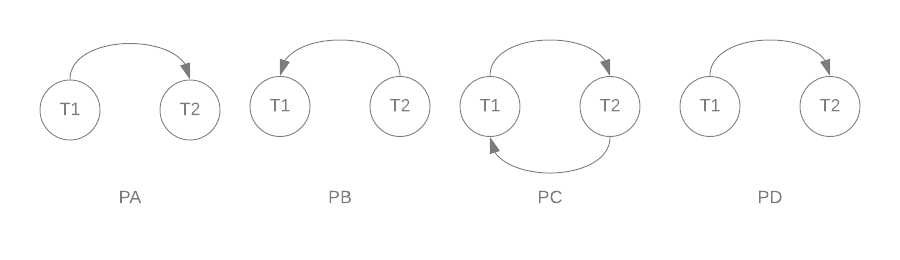
\includegraphics[scale=0.4]{grafo}
\end{center}

\item Dados los Planes PA , PB y PC  dibujar los grafos para probar la serializabilidad por conflictos usando el Algoritmo.

PA: l1(X) ; e1(X) ; l1(Y) ; e1(Y) ; c1; l2(X) ; e2(X) ; c2;

PB: l1(X) ; e1(X) ; l2(X) ; e2(X) ; c2; l1(Y) ; e1(Y) ; c1;

PC: l1(X) ; l2(X) ; e1(X) ; e2(X) ; c2; l1(Y) ; e1(Y) ; c1;

\end{enumerate}